\section{振动解}\label{sec:07.02}

本节从动力学基本方程来求解在弹性力作用下的运动。现在
% 202.jpg

\noindent
还是先讨论系在弹簧一端的质点(图\ref{fig:07.01}),它称为振子。按牛顿第
二定律,振子的运动方程为:
\begin{equation*}
  m \frac { \dif ^ { 2 } x } { \dif t ^ { 2 } } = - k x
\end{equation*}
或者
\begin{equation}\label{eqn:07.02.01}
  \frac { \dif ^ { 2 } x } { \dif t ^ { 2 } } + \frac { k } { m } x = 0
\end{equation}
由于$ k $,$ m $都是正数,所以可以定义一个实数$ \omega $,使得
\begin{equation}\label{eqn:07.02.02}
  \omega ^ { 2 } = \frac { k } { m }
\end{equation}
于是,式\eqref{eqn:07.02.01}可写成
\begin{equation}\label{eqn:07.02.03}
  \frac { \dif ^ { 2 } x } { \dif t ^ { 2 } } + \omega ^ { 2 } x = 0
\end{equation}
式\eqref{eqn:07.02.03}就是振子运动的微分方程。它的解是
\begin{equation}\label{eqn:07.02.04}
  x = A \cos \left( \omega t + \varphi _ { 0 } \right)
\end{equation}
其中$ A $,$ \varphi _ { 0 } $是两个任意常数。图\ref{fig:07.05}\;画出了上式的$ x \mathdash t $关系,它清楚
地显示周期运动的特征。这种周期运动叫做简谐振动。
\begin{figure}[h]
  \vspace{1em}
  \centering
  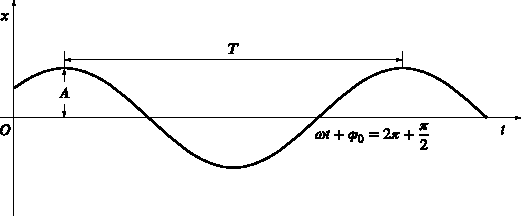
\includegraphics{figure/fig07.05}
  \caption{简谐振动}
  \label{fig:07.05}
  %\vspace{1em}
\end{figure}

现在我们来说明式\eqref{eqn:07.02.04}中各量的物理意义。

首先,由三角函数性质$  \left| \cos \theta \right| \leqslant 1  $ 可知,位移量$ x $的绝对值
% 203.jpg
不能大于$ A $,即
\begin{equation*}
  \begin{aligned}
    \left| x \right| & = \left| A \cos \left( \omega t + \varphi _ { 0 } \right) \right|             \\
                     & = A \left| \cos \left( \omega t + \varphi _ { 0 } \right) \right| \leqslant A
  \end{aligned}
\end{equation*}
这说明$ A $是振子离开平衡位置的最大距离,称为振幅。上节中已
指出,
\begin{equation*}
  x _ { \max } = \sqrt { \frac { 2 E } { k } }
\end{equation*}
所以%\vspace{-1.56em}
\begin{equation*}
  A = \sqrt { \frac { 2 E } { k } }
\end{equation*}
或者%\vspace{-1.56em}
\begin{equation}\label{eqn:07.02.05}
  E = \frac { k } { 2 } A ^ { 2 }
\end{equation}
即振幅的平方与振子的能量成正比。

其次,如果式\eqref{eqn:07.02.04}中的时间$ t $增加一个数值$ \dfrac { 2 \uppi } { \omega } $,$ x $
变成
\begin{equation*}
  \begin{aligned}
    x & = A \cos \left[ \omega \left( t + \frac { 2 \uppi } { \omega } \right) + \varphi _ { 0 } \right] \\
      & = A \cos \left( \omega t + 2 \uppi + \varphi _ { 0 } \right)                                     \\
      & = A \cos \left( \omega t + \varphi _ { 0 } \right)
  \end{aligned}
\end{equation*}
也就是说,相隔$ \dfrac { 2 \uppi } { \omega } $的两个时刻,运动状态是相同的,即运动是
以$ \dfrac { 2 \uppi } { \omega } $为间隔重复的。所以 $ \dfrac { 2 \uppi } { \omega } $就是振动的周期$ T = \dfrac { 2 \uppi } { \omega } $。

又因$ \omega ^ { 2 } = \dfrac { k } { m } $,故有
\begin{equation}\label{eqn:07.02.06}
  T = - \frac { 2 \uppi } { \omega } = 2 \uppi \sqrt { \frac { m } { k } }
\end{equation}
可见,周期仅由振子的质量$ m $和弹簧的弹性系数$ k $来确定,而与振
子的能量$ E $无关,这是简谐振动的重要特征。振子在单位时间内
% 204.jpg
的振动次数,称为频率$ \nu $,由下式给定:
\begin{equation*}
  v = \frac { 1 } { T } = \frac { \omega } { 2 \uppi } = \frac { 1 } { 2 \uppi } \sqrt { \frac { k } { m } }
\end{equation*}
所以
\begin{equation*}
  \omega = 2 \uppi \nu = \frac { 2 \uppi } { T }
\end{equation*}
$ \omega $称为圆频率,它和频率$ \nu $相差一个因子$ 2 \uppi $。

再则,由式\eqref{eqn:07.02.04}可见,当振幅$ A $、圆频率$ \omega $一定时,位置
只决定于$ \left( \omega t + \varphi _ { 0 } \right) $,也就是说振动物体的运动状态可由$ \left( \omega t + \varphi _ { 0 } \right) $
来标志。$ \left( \omega t + \varphi _ { 0 } \right) $这个量叫做位相。知道了位相也就知道了物
体的运动状态。例如,当位相为$ \dfrac { \uppi } { 2 } $,或者$ \dfrac { \uppi } { 2 } + 2 \uppi n $(其中$ n $为整
数)时,就必有$  x = 0   $。

常数$ \varphi _ { 0 } $是时间$  t = 0   $时的位相,所以叫做初位相,它决定$  t = 0  $
时刻振子的位置$  x _ { 0 } = A \cos \varphi _ { 0 }  $。

对式\eqref{eqn:07.02.04}作$ t $的微分,就得到振子速度的表达式
\begin{equation}\label{eqn:07.02.07}
  v = \frac { \dif x } { \dif t } = - \omega A \sin \left( \omega t + \varphi _ { 0 } \right)
\end{equation}

可见,速度的周期变化也由三角函数描写。

对比式\eqref{eqn:07.02.04}与式\eqref{eqn:07.02.07},可以看到,当$ x $到达极大或极
小值时,即$  x = \pm A   $,则速度为零,$  v = 0   $;而当速度达到极大或极小
值时,即$  v = \pm \omega A   $,则位置为零,$  x = 0   $。其实这个性质很容易从
势能曲线(图74)得到。对于能量为$ E $的振子,它的机械能守恒
方程是
\begin{equation*}
  \frac { 1 } { 2 } m v ^ { 2 } + \frac { 1 } { 2 } k x ^ { 2 } = E
\end{equation*}
因此,当
\begin{equation*}
  x =
  \begin{cases}
    A \\
    -A
  \end{cases}
  =
  \begin{cases}
    x _ { \text { max } } \\
    x _ { \text { min } }
  \end{cases}
\end{equation*}
% 205.jpg
\clearpage\noindent
势能等于总能量,$  E = V   $,故动能为零,即速度为零。相反,当速
度达到极值,即动能达到极大时,动能等于总能,势能为零,故
$ x = 0   $。
